\chapter{Janus}
In this chapter, we will illustrate how our tool \LTLfToDFA presented in Chapter \ref{ch:ltlf2dfa} can be efficiently employed in the field of Business Process Management, with particular attention to Process Mining. First of all, we will formally describe the theoretical framework of declarative process mining, introducing a new theorem that generalizes the concept of separated formulas only for \declare constraints. Then, in this context, we will thoroughly describe the implementation of the Janus algorithm \citep{cecconi2018interestingness} for computing the interestingness degree of traces in real event logs. Finally, we will provide such a computation for a real log as an example. 
\section{Declarative Process Mining}
In this section, we will present the theoretical framework of Business Process Management focusing our attention to declarative process mining. We will extend what described in Chapter \ref{ch:theory} providing all additional concepts, definitions and theorems necessary to clearly understand the context.

Business Process Management (BPM) deals with discovering, modeling, analyzing and managing business processes in order to measure their productivity and to improve their performance. These tasks are carried out thanks to logging facilities that, nowadays, all BPM systems have. The extraction and the validation of temporal constraints from event logs (i.e. multi-sets of finite traces) are techniques consisting declarative process mining \citep{montali2010declarative}. Temporal constraints are expressed using \LTLf and/or \PLTL and refers to activities present in traces. In the following, we will formally introduce what event logs and \declare \citep{pesic2008constraint} are. Another important aspect to notice is that these constraints are meant to be checked upon the activation satisfying specific conditions. For these reasons, they are referred as \emph{reactive constraints}.
\paragraph{Event Logs}
The event log is a collection of meaningful data that is the entry point for the consequent process mining. Formally, we consider this meaningful data expressed as a multiple traces containing a sequence of events belonging to the alphabet of symbols $\Sigma$. A single trace can be represented as $t = \tup{e_1,e_2,\dots,e_n}$ where $e_i$ is the event occurring at instant $i$ and $n \in \mathbb{N}$ is the length of the trace $t$.  Now, we can give the following definition:
\begin{definition}
An event log $\L$ is defined as $\L = \{t_1,\dots,t_m\} \in \mathbb{M} (\Sigma^*)$ is a multi-set of traces $t_j$ with $1 \le j \le m$, where $m \in \mathbb{N}$.
\end{definition}
To better indicate the \textit{multiplicity} of traces in $\L$, we can denote it as a superscript compacting the notation. For example, $t_{2}^{10}$ stands for trace $t_2$ occurs $10$ times in $\L$.
\begin{example}\label{ex:traces}
$\L = \{t_{1}^{25},t_{2}^{10},t_{3}^{15},t_{4}^{20},t_{5}^{5},t_{6}^{10}\}$ is an event log of $85$ traces, defined over the alphabet $\Sigma = \{a,b,c,\dots, i \} $. In $ \L $ we have the following traces:
\begin{align*}
t_1 &= \tup{d,f,a,f,c,a,f,b,a,f}\\
t_2 &= \tup{f,e,d,c,b,a,g,h,i}\\
t_3 &= \tup{a,d,a,a,a,a,a,a,a,a,a,a,a,a,a,a,a,a,a,a,a,c}\\
t_4 &= \tup{d,b,a,e}\\
t_5 &= \tup{a,d,a,c,a}\\
t_6 &= \tup{b,c,d,e}
\end{align*}
\end{example}
Furthermore, the event $e_i$ occurring at instant $i$ is denoted by $t(i)$, whereas the segment of $t$ (i.e. the sub-trace) ranging from instant $i$ to instant $j$, where $1 \le i \le j \le n$ is denoted by $t_{[i:j]}$.

Apart from the formal model of event logs, we have real-world event logs that are logs with real data coming from different kind of data sources (e.g. databases, transaction logs, audit log, etc.). All available tools are evaluated against real-world logs. In practice, as we will see in the Section \ref{sec:janus-implementation}, the main way of representing real logs is the XES Standard\footnote{http://www.xes-standard.org}, which is based on the well known XML.
\paragraph{\declare}
\declare is a language concerning declarative process modeling \citep{pesic2008constraint} and consisting of standard templates based on \citep{dwyer1999patterns} that was introduced to simplify the complexity of constraints semantics. Indeed, \declare constraints are expressed in \LTLf, but we will extend \LTLf with Past temporal operators (\LTLp) for capturing also past modalities. In Figure \ref{fig:declare-constraints}, we can see what are the corresponding \LTLf or \LTLp formulas for the most important \declare constraints. 
\begin{figure}[h]
\centering
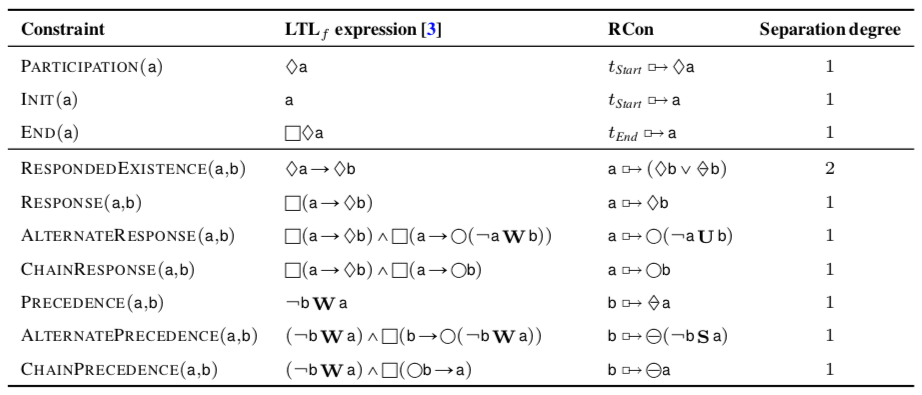
\includegraphics[width=\textwidth]{images/declare-constraints}
\caption{The most important \declare constraints expressed as \LTLf/\PLTL formulas and \emph{reactive constraints.}}
\label{fig:declare-constraints}
\end{figure}
Parameters in a template define tasks and they occurs as events in traces. In Example \ref{ex:declare-examples} we provide a glimpse of \declare patterns.
\begin{example}\label{ex:declare-examples}
Interesting \declare templates \citep{maggi2013knowledge}
\begin{itemize}
\item \textsc{Precedence}(a,b) means \emph{if b occurs then a occurs before b}.
\item \textsc{Responce}(a,b) means \emph{if a occurs then eventually b occurs after a}.
\item \textsc{ChainPrecedence}(a,b) means \emph{the occurrence of b imposes a to occur immediately before}.
\item \textsc{AlternateResponce}(a,b) means \emph{if a occurs then eventually
b occurs after a without other occurrences of a in between}.
\end{itemize}
\end{example}
In addition, one can create his own 	\declare patterns tailored for his purposes. In this way, the \declare standard template can be customized.

A given \declare constraint is verified over traces and those traces \emph{satisfy} it if they do not \emph{violate} it. Here, it is important to notice that these constraints are prone to the principle of \textit{ex falso quod libet}, namely they can be satisfied even without being activated. This represents a big issue for process mining because mining techniques might misunderstand the actual behavior of a process. The solution to this problem is to compute whether a constraint is satisfied or not only upon activation. However, we will see later how to overcome this problem in the Section \ref{sec:janus}.

Now, we give some definitions:
\begin{definition}\citep{gabbay1989declarative}\label{def:pure-temp-formula}
Given an \LTLp formula $\varphi$, we call it \emph{pure past} formula ($\varphi^\blacktriangleleft$) if it consists of only past operators; \emph{pure present} formula ($\varphi^\blacktriangledown$) if it has not any temporal operators; \emph{pure future} formula ($\varphi^\blacktriangleright$) if it consists of only future operators.
\end{definition}
\begin{example}\label{ex:pure-formulas-examples}
Pure formulas:
\begin{itemize}
\item $\boxminus(a \Rightarrow \Once b)$ is a \textbf{pure past} formula;
\item $a \Rightarrow (b \lAND c)$ is a \textbf{pure present} formula
\item $\Box(a \Rightarrow \Next b)$ is a \textbf{pure future} formula
\end{itemize}
\end{example}
The separation of an \LTLp formula to pure past/present/future formulas allows to conduct the analysis on sub-traces (i.e. one referring to the past and the other referring to the future) upon the activation. This is also known as bi-directional on-line analysis. To this extent, we rely on the Separation Theorem stated as follows:
\begin{theorem}\citep{gabbay1989declarative}\label{th:separation-theorem}
Any propositional temporal formula $\varphi$ can be rewritten as a boolean combination of pure temporal formulas.
\end{theorem}
Therefore, following Theorem \ref{th:separation-theorem}, we can give the Definition of \textit{separated formula} as follows:
\begin{definition}\citep{cecconi2018interestingness}\label{def:separated-formula}
Let  $\varphi$ an \LTLp formula over $\Sigma$. A temporal separation is a function $\S: \textsc{ltl}p_f  \rightarrow 2^{\textsc{ltl}p_f \times \textsc{ltl}p_f 	\times \textsc{ltl}p_f}$ such that: $\S(\varphi) = \{(\varphi^{\blacktriangleleft},\varphi^{\blacktriangledown},\varphi^{\blacktriangleright})_1,\dots,\\(\varphi^{\blacktriangleleft},\varphi^{\blacktriangledown},\varphi^{\blacktriangleright})_m\}$ such that:
\begin{equation}\label{eq:separated-formulas}
\varphi \equiv \bigvee^{m}_{j=1} (\varphi^{\blacktriangleleft} \lAND \varphi^{\blacktriangledown} \lAND \varphi^{\blacktriangleright})_j
\end{equation}
where $\varphi^\blacktriangleleft$, $\varphi^\blacktriangledown$ and $\varphi^\blacktriangleright$ are pure formulas over $\Sigma$ as in Definition \ref{def:pure-temp-formula}.
\end{definition}
Notice that Equation \ref{eq:separated-formulas} is a disjunction of conjunction. Moreover, each triple consisting the image function of $\S(\varphi)$ is generally called \emph{separated formula}. In the following, we give an example of separated formula.
\begin{example}\label{ex:separated-formulas}
The separated formulas for $(\Yesterday a \lOR \Diamond b$):
\begin{align*}
(\Yesterday a \lAND True \lAND True)\bigvee(True \lAND True \lAND \Diamond b)
\end{align*}
\end{example}
PUT HERE THE NEW GENERALIZATION OF THE THEOREM

Since the Janus algorithm relies on the construction of the automata for separated \LTLp formulas, we will refer to notions explained previously in Section \ref{sec:formula-to-automa}. The crucial point is that given a separated \LTLp formula $\varphi$ we can build a minimum \DFA that \emph{accepts} all and only the traces satisfying formula $\varphi$.

In the following sections, we will describe in details the Janus approach giving fundamentals definitions and theorems. Then, we will illustrate the algorithm and its practical implementation.
\section{Janus}\label{sec:janus}
Declarative process modeling defines a list of \declare constraints to be satisfied during the execution of the process model. These constraints are of a reactive nature in the sense that the occurrence of some task bounds the occurrence of other activities. As anticipated in the previous Section, this kind of behavior might lead to the principle of \textit{ex falso quod libet}, namely a constraint can be satisfied even though it is never activated. Here, the Janus approach \citep{cecconi2018interestingness} solves this problem allowing the user to indicate the activation condition for the constraint directly in the constraint formula. In this way, constraints are activated only if the activation condition holds. Therefore, we can refer to these constraints as \textit{reactive constraints} (\rcon).
\begin{definition}
Given an alphabet $\Sigma$, let $\alpha \in \Sigma$ be an \emph{activation} and $\varphi$ be an \LTLp formula over $\Sigma$. A Reactive Constraint (\rcon) $\Psi$ is a pair $(\alpha, \varphi)$, denoted as $\Psi \doteq \alpha \boxright \varphi$
\end{definition}
\subsection{Algorithm}
\section{Implementation}\label{sec:janus-implementation}
\subsection{Package Structure}
\subsection{Classes}
\section{Summary}